This chapter presents the methodology, experiments, and results of the two core pipelines developed in this project: the Design-to-Code Pipeline and the RAG-based Knowledge Base. For each pipeline, we describe the approach taken, the algorithms and iterations involved, and the evaluation methods used to validate the results.

%% ============================================================
%%  PART A: DESIGN-TO-CODE PIPELINE
%% ============================================================

\section{Design-to-Code Pipeline}

\subsection{Setup and Tooling}

The Design-to-Code pipeline was built around Claude Code (Anthropic's AI coding agent, using the Opus model) as the central orchestrator, connected to two Model Context Protocol (MCP) servers that provide it with external tool access:

\begin{itemize}
    \item \textbf{Figma Desktop MCP Server:} Exposes live Figma design metadata in a machine-readable format. Rather than using Figma's REST API (which requires token management and returns static snapshots), the Desktop Bridge plugin connects via WebSocket to the open Figma file, allowing Claude to read component properties, variants, colors, spacing, typography, and icons in real time.
    
    \item \textbf{Chrome DevTools MCP Server:} Provides browser automation capabilities, allowing Claude to navigate to Storybook pages, take screenshots, inspect computed styles, click interactive elements, and compare the rendered component against the Figma design.
\end{itemize}

The development environment consisted of the Angular 16 frontend of the Knoccs application, with components generated into \texttt{src/app/shared/components/}. Storybook served as the visual documentation and validation layer, running on \texttt{localhost:9009}. Each generated component produced four to five files: \texttt{.component.ts}, \texttt{.component.html}, \texttt{.component.scss}, \texttt{.types.ts}, and optionally \texttt{.interfaces.ts}.

For the sync workflow, three additional artifacts were configured: \texttt{design\_system\_mapping.json} (which records every Figma node ID alongside its Angular component path and last-synced timestamp), \texttt{sync-figma.js} (a Node.js driver invoked through \texttt{npm run sync:figma <component>}), and \texttt{SYNC\_DESIGN\_SYSTEM\_COMPONENT\_PLAN.md} (the 8-phase rulebook Claude follows during a sync run). These artifacts make the sync pipeline reproducible across the team and remove the need to hand-author prompts for individual sync runs. The sync interface, described in Section~\ref{sec:sync}, sits on top of these artifacts and exposes them through a designer-facing UI.

\subsection{Iterative Instruction Refinement}
\label{sec:prompt-engineering}

The core algorithmic contribution of the Design-to-Code pipeline is the iterative development of a comprehensive instruction file (\texttt{CLAUDE.md}) that governs how Claude generates Angular components from Figma designs. This file evolved through \textbf{nine iterations} (v0 through v8), each addressing failure modes discovered during actual component generation. A parallel set of instructions for Storybook story generation evolved through \textbf{seven iterations}.

\subsubsection{Main Component Generation Instructions}

The evolution of the main \texttt{CLAUDE.md} file followed a clear trajectory from a static style guide to a fully automated, multi-agent, phased pipeline with strict human-in-the-loop governance.

\textbf{Version 0: Baseline Style Guide:} The initial version ($\sim$350 lines) served as a conventional coding standards document. It established the project structure, reference components (Breadcrumb, Toastbar, Snackbar, List), file naming conventions, basic Figma extraction instructions, and Storybook requirements. No agents, phases, or enforcement rules were defined.

\textbf{Version 1: Multi-Agent Architecture:} An expansion ($\sim$770 lines) that introduced eight specialized agents:

\begin{enumerate}
    \item \texttt{figma-extractor}: Extracts design metadata from Figma via MCP
    \item \texttt{component-generator}: Generates Angular component files
    \item \texttt{storybook-generator}: Creates Storybook stories
    \item \texttt{unit-test-generator}: Generates behavioral unit tests
    \item \texttt{design-system-validator}: Validates design token compliance
    \item \texttt{figma-design-verification}: Cross-checks output against Figma
    \item \texttt{angular-code-improver}: Refactors generated code
    \item \texttt{claude-md-compliance-checker}: Ensures instruction compliance
\end{enumerate}

A mandatory agent chain was defined: \texttt{figma-extractor} $\rightarrow$ \texttt{component-generator} $\rightarrow$ \texttt{storybook-generator} $\rightarrow$ \texttt{unit-test-generator} $\rightarrow$ \texttt{claude-md-compliance-checker}. This version also introduced the complete design token system (color scales from \texttt{\$color-0} through \texttt{\$color-100} across 8 palettes), the \texttt{toRem()} function for responsive pixel-to-rem conversion, BEM-like CSS naming conventions, icon system documentation, and typography specifications.

\textbf{Version 2: Phased Pipeline with Human-in-the-Loop:} A rewrite ($\sim$800+ lines) that introduced a seven-phase workflow with strict enforcement rules:

\begin{enumerate}
    \item[\textbf{Phase 0:}] \textbf{EXPLORE}: Extract all variants, states, and properties from Figma via MCP. Present findings to user and wait for confirmation before proceeding.
    \item[\textbf{Phase 1:}] \textbf{DOCUMENT}: Generate a behavior specification (variants, states, sizes, interactions, accessibility) and a Figma-to-Code mapping table covering colors, spacing, typography, icons, borders, effects, and states.
    \item[\textbf{Phase 2:}] \textbf{IMPLEMENT}: Delegate to the \texttt{component-generator} agent to produce the TypeScript, HTML, and SCSS files. Register in \texttt{SharedModule}. Present to user for approval.
    \item[\textbf{Phase 3:}] \textbf{VALIDATE}: Run a seven-section design audit (color, spacing, typography, icon, variant, state, and code quality). Self-correction loop with a maximum of 3 attempts before escalating.
    \item[\textbf{Phase 4:}] \textbf{STORYBOOK}: Generate stories for all Figma variants, including an \texttt{AllVariants} showcase story.
    \item[\textbf{Phase 5:}] \textbf{CHROME MCP}: Visual comparison against Figma via browser screenshots. Behavioral testing of interactive elements. Generate a test report.
    \item[\textbf{Phase 6:}] \textbf{COMPLETE}: Generate unit tests, run compliance checker, and present a final checklist.
\end{enumerate}

Four strict enforcement rules were placed at the top of the document:
\begin{enumerate}
    \item Stop and confirm at every phase gate. Missing response is NOT confirmation.
    \item NEVER fix discrepancies without user approval. If same fix fails twice, escalate.
    \item NEVER use variant values not present in Figma. Flag discrepancies in both directions.
    \item NEVER skip mandatory interaction points.
\end{enumerate}

Nine mandatory stop points were defined where Claude must pause and wait for user input, preventing autonomous decisions that could introduce errors.
\\\\
\textbf{Versions 3--8: Practical Refinements:} Each subsequent version addressed a specific failure mode encountered during real component generation:

\begin{itemize}
    \item \textbf{v3:} Introduced an icon fallback system, if a custom SVG icon fails to render during Chrome MCP verification, fall back to the equivalent Angular Material icon and document the substitution.
    \item \textbf{v4:} Added a sixth rule, NEVER run unit tests (\texttt{ng test}) without explicit user permission. This was added after Claude autonomously triggered test runs that disrupted the development workflow.
    \item \textbf{v7:} Added a component reuse rule, before implementing any UI element inline (e.g., avatar circles, badges), check if a reusable component already exists in \texttt{shared/components/} and use it instead. This addressed Claude re-implementing existing components.
    \item \textbf{v8:} Simplified SCSS import paths from relative (\texttt{../../../../styles/colors}) to short-form (\texttt{@import `colors'}) after configuring \texttt{angular.json} include paths. Deprecated the \texttt{isIconSvg()} pattern in favor of globally registered SVG icons. Added a pitfall warning for Figma documentation pages vs.\ actual component nodes.
\end{itemize}

Table \ref{tab:prompt_evolution} summarizes the evolution across all iterations.

\begin{table}[H]
\centering
\caption{Evolution of the Main CLAUDE.md Instruction File}
\label{tab:prompt_evolution}
\begin{tabular}{|c|c|c|c|c|c|}
\hline
\textbf{Version} & \textbf{Lines} & \textbf{Agents} & \textbf{Phases} & \textbf{Rules} & \textbf{Key Addition} \\ \hline
v0 & $\sim$350 & 0 & 0 & 0 & Baseline style guide \\ \hline
v1 & $\sim$770 & 8 & 0 & 0 & Multi-agent + design tokens \\ \hline
v2 & $\sim$800 & 8 & 7 & 5 & Phased pipeline + human gates \\ \hline
v3 & $\sim$830 & 8 & 7 & 5 & Icon fallback system \\ \hline
v4 & $\sim$850 & 8 & 7 & 6 & Unit test permission rule \\ \hline
v7 & $\sim$855 & 8 & 7 & 6 & Component reuse rule \\ \hline
v8 & $\sim$860 & 8 & 7 & 6 & SCSS simplification + pitfalls \\ \hline
\end{tabular}
\end{table}

\subsubsection{Storybook Generation Instructions}

A parallel instruction file (\texttt{CLAUDE\_STORYBOOK.md}) was developed specifically for generating Storybook stories. It evolved through seven iterations (v0 through v4, plus a discrepancy log and a final consolidated version) and followed a similar trajectory:

\begin{itemize}
    \item \textbf{v0:} Basic 4-step workflow (read component, check existing stories, analyze variants, create story file) with no phases or enforcement.
    \item \textbf{v1:} Major expansion to a 5-phase workflow with Figma integration via Chrome MCP, strict enforcement rules, session state tracking, \texttt{@Output()} event handling with \texttt{action()} from \texttt{@storybook/addon-actions}, and a Figma-to-Browser translation reference for comparing sizing, colors, and borders.
    \item \textbf{v3:} Added SCSS color variable resolution, before labeling variants, Claude must trace each variant's color through the \texttt{\_colors.scss} file to its actual hex value, preventing mislabeling.
    \item \textbf{v4:} Introduced three critical rules: (a) \textit{Code always takes precedence over Figma}: Storybooks render real Angular components, so if code behavior differs from Figma, follow the code; (b) \textit{Verify SCSS color variables before labeling variants}; (c) \textit{Verify icon SVG content before assuming orientation/shape}. Also added mandatory template path tracing, before writing stories, Claude must trace which \texttt{*ngIf} branches will be active for each story's arguments.
    \item \textbf{Discrepancy Log:} A separate file documented 13 observed Figma-to-code discrepancies (e.g., datepicker has no code for error state, chip's three-dot icon is horizontal not vertical, toastbar only has small variants). This empirical log motivated the code-takes-precedence rules.
    \item \textbf{Final Version:} Added Rule 9 (every story must wire args to controls using \texttt{render: (args) =>} with spread into \texttt{props}) and documented 10 known Storybook-Angular rendering pitfalls, including \texttt{::ng-deep} stripping, asset path resolution differences, stateful parent-child binding, and missing sibling component styles.
\end{itemize}

\subsection{Component Generation and Results}

Using the finalized instruction files, 20 Angular components were generated from Figma designs. Table \ref{tab:components} lists all generated components.

\begin{table}[H]
\centering
\caption{Generated Angular Components}
\label{tab:components}
\begin{tabular}{|c|l|c|l|}
\hline
\textbf{\#} & \textbf{Component} & \textbf{\#} & \textbf{Component} \\ \hline
1 & Accordion & 11 & Phone Input \\ \hline
2 & Avatar & 12 & Popup \\ \hline
3 & Breadcrumb & 13 & Radio Button \\ \hline
4 & Button & 14 & Single-Select Dropdown \\ \hline
5 & Checkbox & 15 & Snackbar \\ \hline
6 & Chip & 16 & Stepper \\ \hline
7 & Datepicker & 17 & Tabs \\ \hline
8 & Input & 18 & Toastbar \\ \hline
9 & List & 19 & Toggle \\ \hline
10 & Multi-Select Dropdown & 20 & Tooltip \\ \hline
\end{tabular}
\end{table}

Each component was generated through the full phased pipeline: Figma extraction, behavior specification, code generation, design audit, Storybook story creation, Chrome MCP visual verification, and unit test generation. All generated components and their Storybook stories underwent PR review by the SpurSol development team, with feedback incorporated iteratively. The setup used for each generation session was: Claude Code with Opus 4, session resumption enabled, Chrome MCP and Figma MCP connected, with the specific component's Figma link provided as input.

\subsection{Component Evaluation}

Three complementary evaluation methods were used to validate the quality of generated components.

\subsubsection{CLIP Visual Similarity}

To quantitatively measure the visual fidelity of generated components against their Figma designs, we used OpenAI's CLIP (Contrastive Language--Image Pre-training) model. For each of the 20 components, a screenshot was taken from the Figma design (original) and from the rendered Storybook story (generated). CLIP embeddings were computed for both images, and cosine similarity was calculated between them.

\begin{table}[H]
\centering
\caption{CLIP Visual Similarity Scores per Component}
\label{tab:clip_results}
\begin{tabular}{|l|c||l|c|}
\hline
\textbf{Component} & \textbf{CLIP Score} & \textbf{Component} & \textbf{CLIP Score} \\ \hline
Accordion & 0.899 & Phone Input & 0.808 \\ \hline
Avatar & \textbf{1.000} & Popup & 0.937 \\ \hline
Breadcrumb & 0.894 & Radio Button & 0.655 \\ \hline
Button & 0.758 & Single-Select Dropdown & 0.931 \\ \hline
Checkbox & 0.757 & Snackbar & 0.524 \\ \hline
Chip & 0.720 & Stepper & 0.970 \\ \hline
Datepicker & 0.886 & Tabs & 0.759 \\ \hline
Input & 0.825 & Toastbar & 0.843 \\ \hline
List & 0.740 & Toggle & 0.852 \\ \hline
Multi-Select Dropdown & 0.850 & Tooltip & 0.903 \\ \hline
\multicolumn{4}{c}{} \\ \hline
\textbf{Average} & \textbf{0.826} & \textbf{Median} & \textbf{0.847} \\ \hline
\textbf{Std Dev} & \textbf{0.114} & \textbf{Min / Max} & \textbf{0.524 / 1.000} \\ \hline
\end{tabular}
\end{table}

The average CLIP similarity score of \textbf{0.826} exceeds the 80\% visual similarity target defined in the non-functional requirements (Section \ref{chap:srs}). Components with simpler visual structures (Avatar, Stepper, Popup) scored highest, while components with complex interactive states that render differently in Storybook vs.\ Figma (Snackbar, Radio Button) scored lower. The Snackbar's low score (0.524) is attributed to the fact that only small variants existed in code while Figma showed larger variants, a known discrepancy documented in the Figma-code discrepancy log.

% TODO: Consider adding a bar chart figure of the CLIP scores

\subsubsection{Unit Testing (Behavioral Testing)}

Behavioral unit tests were generated for components using Angular TestBed and Jasmine. The testing strategy was derived from three sources: the Figma specification (visual states), the component API (\texttt{@Input} and \texttt{@Output} contracts), and the behavior rules defined in the \texttt{CLAUDE.md} instructions.

As a representative example, the Checkbox component received 74 automated tests across 15 categories:

\begin{table}[H]
\centering
\caption{Unit Test Breakdown for the Checkbox Component (74 Tests)}
\label{tab:unit_tests}
\begin{tabular}{|l|c|p{7cm}|}
\hline
\textbf{Category} & \textbf{Tests} & \textbf{What it Verifies} \\ \hline
Component Creation & 2 & Instantiation and root element rendering \\ \hline
Input Defaults & 4 & Default values for label, checked, indeterminate, disabled \\ \hline
State Getter & 8 & All 5 states return correctly, priority edge cases \\ \hline
onClick Behavior & 4 & State transitions: Inactive$\rightarrow$Active, Active$\rightarrow$Inactive, Partial$\rightarrow$Active \\ \hline
Disabled Suppression & 3 & Click does nothing when disabled \\ \hline
Space Key & 3 & Space triggers onClick, calls preventDefault \\ \hline
Other Keys Ignored & 4 & Enter, Tab, Escape, ArrowDown don't trigger \\ \hline
@Output Emission & 6 & Emits correct payload, doesn't emit when disabled \\ \hline
CSS Classes & 9 & Correct modifier class per state \\ \hline
Label Rendering & 5 & Label shows/hides, displays correct text \\ \hline
Checkmark Icon & 6 & Icon present in active/check-disabled states only \\ \hline
Dash Element & 6 & Dash present in partial state only \\ \hline
ARIA Attributes & 9 & role, aria-checked, aria-disabled, tabindex \\ \hline
isIconSvg Helper & 2 & SVG icon detection \\ \hline
DOM Click Binding & 3 & Template click binding triggers correctly \\ \hline
\end{tabular}
\end{table}

The tests act as behavioral contracts: they verify \textit{what} the component does (observable behavior) rather than \textit{how} it works internally. Visual/CSS testing was intentionally excluded from unit tests as it is covered by Storybook visual verification. Integration testing (component inside a parent form) was deferred as a separate concern.

\subsubsection{Visual Verification through Storybook and Chrome MCP}

The third evaluation method used Chrome MCP to perform automated visual comparison during Phase 5 of the generation pipeline. For each component, Claude navigated to the Storybook iframe URL, took screenshots of every story variant, and compared them against the corresponding Figma frames. This process also included:

\begin{itemize}
    \item \textbf{Console Error Checking:} Verifying no Angular runtime errors (e.g., \texttt{NG05105}, \texttt{NullInjectorError}) appear during rendering.
    \item \textbf{Interactive Element Testing:} Testing dropdowns, expandable sections, hover states, disabled states, and form inputs through Chrome MCP's click and hover commands.
    \item \textbf{Computed Style Verification:} Using \texttt{chrome.evaluate()} to inspect rendered CSS values and compare against expected design tokens.
\end{itemize}

\subsection{Component Mapping}

All 20 generated components were mapped between Figma and code in a \\ \texttt{design\_system\_mapping.json} configuration file. Each entry contains:

\begin{itemize}
    \item \textbf{codePath:} The path to the Angular component folder relative to \texttt{ClientApp/}
    \item \textbf{figmaPath:} An array of Figma URLs (with node IDs) pointing to the component's design frames
    \item \textbf{lastSynced:} A timestamp tracking the last synchronization date
\end{itemize}

This mapping serves as the foundation for the sync pipeline described in the next section, enabling automated detection of which code files correspond to which Figma designs.

\subsection{Figma-to-Code Sync Pipeline}
\label{sec:sync}

A key contribution of this project is the development of a sync pipeline that keeps Angular component code in sync with evolving Figma designs. Instead of regenerating components from scratch when designs change, the sync pipeline detects differences and applies targeted updates.

\subsubsection{Sync Architecture}

The sync pipeline operates through the following workflow:

\begin{enumerate}
    \item The developer runs \texttt{npm run sync:figma [component-name]}, which triggers a Node.js script (\texttt{sync-figma.js}).
    \item The script reads \texttt{design\_system\_mapping.json}, generates a \texttt{sync-task.json} file containing the component name and Figma URLs, and produces a \texttt{prompt.txt} file.
    \item The developer launches Claude Code with the generated prompt.
    \item Claude follows an 8-phase sync workflow:
\end{enumerate}

\begin{table}[H]
\centering
\caption{Sync Pipeline Phases}
\label{tab:sync_phases}
\begin{tabular}{|c|l|p{8cm}|}
\hline
\textbf{Phase} & \textbf{Name} & \textbf{Description} \\ \hline
0 & LOAD & Read sync-task.json, acknowledge component and Figma links \\ \hline
1 & ANALYZE & Read Figma via MCP, extract all specs (colors, spacing, typography, icons, variants) \\ \hline
2 & COMPARE & Read existing code, generate diff report, present to user for approval \\ \hline
3 & APPLY & User confirms changes, backup files, apply SCSS/TS/HTML/story updates \\ \hline
4 & VALIDATE & Code audit: no hex colors, no raw px values, icon consistency check \\ \hline
5 & TEST & User starts Storybook, Chrome MCP screenshots, comparison report \\ \hline
6 & PR & Create git branch, commit changes, push, create pull request via \texttt{gh} \\ \hline
7 & COMPLETE & Summary and cleanup log \\ \hline
\end{tabular}
\end{table}

\subsubsection{Sync Testing and Results}

The sync pipeline was tested with multiple components:

\begin{itemize}
    \item \textbf{Toggle (color change):} A simple color token change in Figma was detected and synced correctly via the pipeline.
    \item \textbf{Accordion (discrepancy detection):} Without changing anything in Figma, the pipeline was run to detect existing discrepancies between code and design. It detected several issues but consistently missed spacing differences, requiring manual intervention to point out the missed changes.
    \item \textbf{Popup (full sync):} A complete sync was performed successfully through Figma Desktop MCP.
\end{itemize}

The sync system achieves approximately \textbf{80--90\% automation}, with the remaining 10--20\% requiring human judgment for: approving changes, resolving ambiguous Figma designs, handling icon name mismatches between Figma naming conventions and the codebase's \texttt{ICON\_NAMES} constants, and addressing complex component logic changes that extend beyond visual properties. Both Figma Desktop MCP and Figma Console MCP were tested, with similar results, both struggled with spacing detection but performed well on color, variant, and structural changes.

\subsubsection{Sync Interface}

To make the sync pipeline accessible to designers (the primary maintainers of the design system), an interface was built on top of the sync artifacts described in Section~\ref{sec:sync}. The interface reads \texttt{design\_system\_mapping.json}, presents all registered components in a dropdown, and assembles the corresponding sync prompt automatically so that designers do not need to construct prompts manually. Sync status and last-synced timestamps are surfaced in the UI, and the underlying CLIP evaluation script can be triggered from the same interface to verify the resulting Storybook output against the updated Figma frame. The end-to-end flow, component selection, sync execution, validation, and pull-request creation, is therefore reachable without leaving the interface.

\begin{figure}[H]
    \centering
    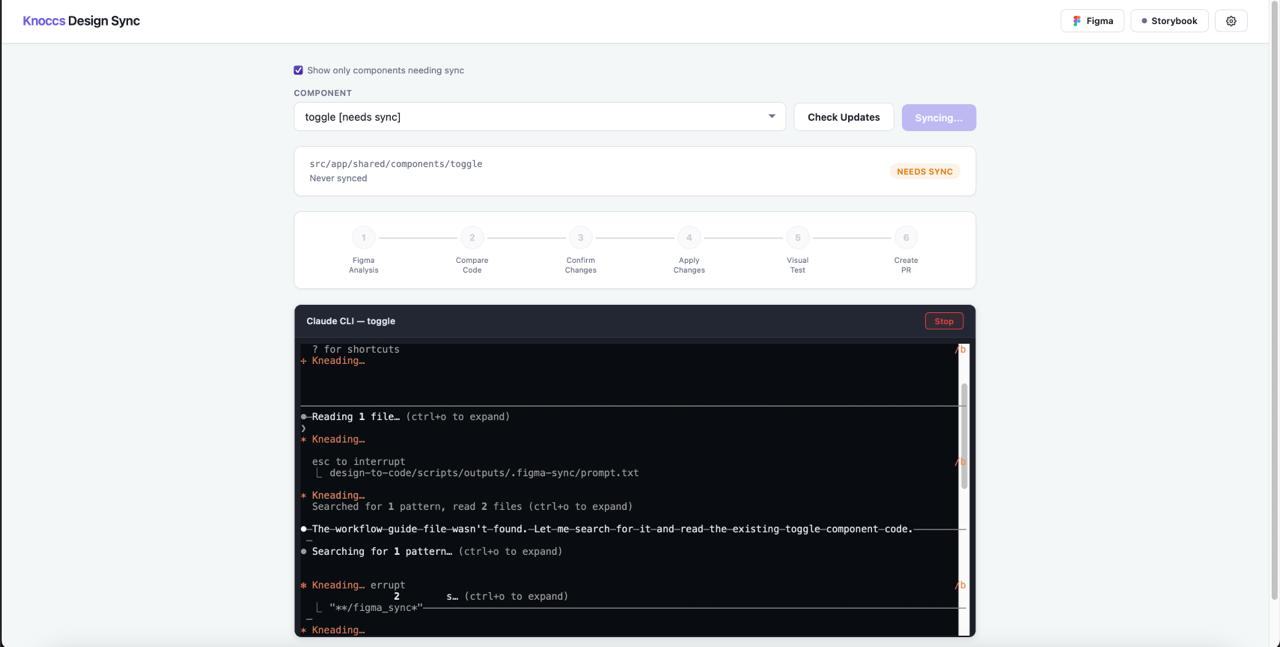
\includegraphics[width=0.9\linewidth]{figures/methodology/interface.jpeg}
    \caption{Sync Interface}
    \label{sync_interface}
\end{figure}


\subsection{Feature Validation: Tag and Macro Management}

To validate that the generated component library could be used to build real features within Knoccs, two feature modules were implemented: Tag Management and Macro Management.

\subsubsection{Approach}

A separate \texttt{CLAUDE.md} file was created for the Knoccs codebase (distinct from the component generation instructions) that provided Claude with full context about the existing architecture: the three-tier Repository Pattern (Controller $\rightarrow$ Business Logic $\rightarrow$ Repository $\rightarrow$ Database), and the Angular frontend structure. Existing Knoccs screens were used to test how the generated components integrate within real pages and workflows.

For each feature:
\begin{enumerate}
    \item A requirements document was simplified into a prompt for Claude.
    \item Reference features from the existing codebase (e.g., Email Creation) were provided as architectural examples.
    \item Claude generated the frontend using components from the generated library, and the backend following the Repository Pattern with C\# models, repositories, controllers, and services.
    \item The generated code was validated for functional accuracy and integration feasibility.
\end{enumerate}

\subsubsection{Results}

Tag Management and Macro Management were implemented end-to-end using the generated component library and the Repository Pattern backend, demonstrating that the Design-to-Code pipeline produces components that are functionally suitable for production feature development. Both modules pass functional validation in the development environment; final integration and rollout into the live Knoccs deployment remain in progress with the SpurSol team. The backend agents followed the existing Knoccs architecture, producing C\# models, repositories, controllers, and services consistent with the codebase conventions.

%% ============================================================
%%  PART B: RAG PIPELINE
%% ============================================================

\section{RAG-based Knowledge Base}

\subsection{Architecture Overview}

The RAG (Retrieval-Augmented Generation) system follows a two-pipeline architecture: an offline \textbf{Data Ingestion Pipeline} that processes and indexes documents, and an online \textbf{Data Inference Pipeline} that handles user queries in real time.

The technology stack consists of:
\begin{itemize}
    \item \textbf{Backend Framework:} FastAPI with Uvicorn
    \item \textbf{Orchestration:} LangChain
    \item \textbf{Vector Store:} PostgreSQL with pgvector extension (hosted on Supabase)
    \item \textbf{Embedding Model:} \texttt{all-mpnet-base-v2} (Sentence Transformers, 768-dimensional)
    \item \textbf{Re-ranking Model:} \texttt{cross-encoder/ms-marco-MiniLM-L-6-v2}
    \item \textbf{LLM:} GPT-4o (temperature 0.1)
    \item \textbf{Evaluation:} DeepEval with GPT-4o-mini as the evaluation model
\end{itemize}

The complete RAG architecture is illustrated in Figure \ref{fig:rag_architecture_diagram}.

\subsection{Data Ingestion Pipeline}

The ingestion pipeline converts raw documents into vector embeddings stored in PostgreSQL. The process operates in three stages:

\subsubsection{Data Loading}

Documents are loaded from a data directory using LangChain community loaders, supporting multiple formats: \texttt{PyPDFLoader} for PDFs, \texttt{Docx2txtLoader} for DOCX, \texttt{TextLoader} for TXT, \texttt{UnstructuredExcelLoader} for XLSX, \texttt{CSVLoader} for CSV, and \texttt{JSONLoader} for JSON files. Metadata files (company information and employee records) are loaded into relational PostgreSQL tables rather than being vectorized, preserving their structured nature for lookup queries.

A key design decision was the \textbf{grouping of small documents by company}. Emails, conversations, notes, and tasks, which individually are too small to form meaningful chunks, are aggregated into single LangChain \texttt{Document} objects per company. This ensures each company's records form a coherent context rather than thousands of tiny, context-poor fragments. Larger documents (PDFs, DOCX) remain as individual documents, with company ownership inferred from filename matching against the companies table.

The knowledge base comprised data from \textbf{10 companies}, totaling approximately \textbf{56 files} including service agreements, HR policies, leave/attendance policies, company overviews, NDAs, annual reports, memos, and structured data (emails, conversations, notes, tasks).

\subsubsection{Chunking Strategy}

Documents are split using LangChain's \texttt{RecursiveCharacterTextSplitter} with a hierarchy of nine separators, from triple newlines down to individual characters. The default configuration uses a \textbf{chunk size of 1,024 characters} with a \textbf{256-character overlap} to maintain context across chunk boundaries.

Before chunking, PDF-specific preprocessing removes noise: standalone page numbers, excessive whitespace, hyphenation at line breaks, and lines with less than 30\% alphanumeric content. After chunking, two quality filters are applied:

\begin{itemize}
    \item Chunks shorter than 50 characters are discarded.
    \item Chunks with less than 60\% alphanumeric and space content are discarded.
\end{itemize}

A section header detection heuristic identifies numbered sections, ALL-CAPS headings, lines ending with colons, and title-case short lines. The detected section name is stored in each chunk's metadata, enabling section-aware retrieval. Every chunk inherits metadata including \texttt{company\_id}, \texttt{source}, \texttt{name}, \texttt{type}, \texttt{chunk\_id}, and \texttt{section} from its parent document.

\subsubsection{Embedding and Indexing}

Text chunks are encoded into 768-dimensional vectors using the \texttt{all-mpnet-base-v2} Sentence Transformer model. The vectors are stored in PostgreSQL using the \texttt{pgvector} extension with an \textbf{IVFFlat index} configured with cosine distance operations \\ (\texttt{vector\_cosine\_ops}) and 100 lists. Additional B-tree indexes on \texttt{company\_id} columns enable efficient company-scoped queries.

The database schema consists of six tables:

\begin{table}[H]
\centering
\caption{RAG Database Schema}
\label{tab:rag_schema}
\begin{tabular}{|l|p{9cm}|}
\hline
\textbf{Table} & \textbf{Purpose} \\ \hline
\texttt{companies} & Company metadata (ID, name, domain) \\ \hline
\texttt{documents} & Document records with company FK, name, type, source \\ \hline
\texttt{chunks} & Text chunks with document FK, company FK, section metadata \\ \hline
\texttt{embeddings} & 768-dim vectors with chunk FK (unique), company FK \\ \hline
\texttt{internal\_employees} & Knoccs employee records (name, email, role) \\ \hline
\texttt{external\_employees} & Client-side contacts with company FK \\ \hline
\end{tabular}
\end{table}

\subsection{Data Inference Pipeline}

The inference pipeline handles real-time user queries through a four-stage process: company identification, hybrid retrieval, cross-encoder re-ranking, and LLM-grounded response generation.

\subsubsection{Company Identification}

All queries are scoped to a single company to enforce \textbf{data isolation}, the system never returns information from one company's data in response to a query about another. Company extraction uses three methods in order of priority:

\begin{enumerate}
    \item \textbf{Exact/fuzzy string matching:} Company names in the query are matched against the database using \texttt{difflib.SequenceMatcher} with a similarity threshold of 0.6.
    \item \textbf{Employee name lookup:} If no company name is found, person names are extracted via regex and looked up in the employee tables to identify their associated company.
    \item \textbf{Conversation history fallback:} If neither method succeeds, previous messages in the conversation are scanned for previously mentioned companies.
\end{enumerate}

If no company can be identified through any method, the query is rejected with a message asking the user to specify the company.

\subsubsection{Hybrid Retrieval}

Retrieval operates in three stages, all scoped to the identified \texttt{company\_id}:

\textbf{Stage 1: Dual Retrieval:}
\begin{itemize}
    \item \textbf{BM25 Keyword Search:} All chunks for the target company are loaded from PostgreSQL, tokenized in memory, and scored using Okapi BM25 (from the \texttt{rank\_bm25} library). The top $k/2$ results are returned with scores normalized relative to the maximum.
    \item \textbf{Dense Vector Search:} The query is encoded using the same embedding model, and a cosine distance query (\texttt{<=>} operator) is executed against the \texttt{embeddings} table filtered by \texttt{company\_id}, returning the top $k/2$ results.
\end{itemize}

\textbf{Stage 2: Merge and Deduplicate:} Results from both retrievers are combined. Duplicate chunks (same \texttt{chunk\_id}) are removed, and the set is trimmed to $k$ candidates (default $k = 50$).

\textbf{Stage 3: Cross-Encoder Re-ranking:} All candidate (query, chunk\_text) pairs are scored by the \texttt{cross-encoder/ms-marco-MiniLM-L-6-v2} model. Results are sorted by re-rank score in descending order, and the top 15 are selected for context assembly.

This three-stage hybrid approach combines the complementary strengths of keyword matching (effective for exact terms like ticket IDs, client names, and contract numbers) and semantic search (effective for paraphrased or conceptual queries), with a cross-encoder providing a final quality filter that considers the full interaction between query and passage.

\subsubsection{Response Generation}

The top-ranked chunks are assembled into a prompt context alongside the user's query, conversation history, and a system prompt. The system prompt instructs GPT-4o to:

\begin{itemize}
    \item Identify itself as the ``Knoccs AI Assistant''
    \item Enforce strict data isolation per company
    \item Format responses in Markdown (headers, bullet points, bold, tables)
    \item Synthesize information naturally across multiple retrieved documents without meta-references (e.g., not ``According to Document 1\ldots'')
    \item Include source citations for traceability
\end{itemize}

The temperature is set to 0.1 for factual, deterministic responses. Conversation history is maintained across queries, and when it exceeds 10 messages, older messages are summarized by the LLM into 2--3 sentences to maintain context without exceeding token limits.

\subsection{Server Architecture}

The RAG system is deployed as a standalone FastAPI server with the following endpoints:

\begin{table}[H]
\centering
\caption{RAG Server API Endpoints}
\label{tab:rag_endpoints}
\begin{tabular}{|l|l|p{7.5cm}|}
\hline
\textbf{Method} & \textbf{Path} & \textbf{Purpose} \\ \hline
GET & \texttt{/health} & Health check (DB connectivity, KB status) \\ \hline
POST & \texttt{/rag/query} & Main query endpoint (accepts query, top\_k, conversation history) \\ \hline
POST & \texttt{/rag/evaluate} & Run DeepEval metrics on a query \\ \hline
GET & \texttt{/rag/stats} & Knowledge base statistics \\ \hline
POST & \texttt{/rag/rebuild} & Full KB rebuild (clear + reload + re-embed) \\ \hline
DELETE & \texttt{/rag/clear} & Clear all data from the vector store \\ \hline
\end{tabular}
\end{table}

The integration with the main Knoccs platform follows a proxy architecture: the Angular frontend communicates with the C\# .NET backend via REST APIs, which then forwards RAG queries to the FastAPI server via an HTTP client wrapper. The .NET layer injects company context from the authenticated user's session, ensuring data isolation is enforced at the application level as well. The frontend never calls the RAG server directly.

\subsection{RAG Frontend Integration}

The RAG interface was integrated into the Knoccs sidebar as a ``RAG Document Assistant'' (visible under AI Features). The interface provides:

\begin{itemize}
    \item A conversational chat interface for natural-language queries
    \item Markdown-rendered responses with structured formatting
    \item Source citations with unique deduplication (each source shown only once)
    \item Document upload capability for expanding the knowledge base
    \item A company-specific dropdown for scoping queries
    \item Online/offline status indicator for the RAG server
    \item Multi-turn conversation support with context retention
\end{itemize}

Design consistency was maintained by Eman, ensuring the RAG interface follows the same design patterns as the rest of the Knoccs application.

\subsection{RAG Evaluation with DeepEval}

\subsubsection{Evaluation Framework}

The RAG system was evaluated using DeepEval, an open-source evaluation framework with native RAG support. Three metrics were used, each scored from 0 to 1 with a pass/fail threshold of 0.7:

\begin{enumerate}
    \item \textbf{Answer Relevancy:} Measures whether the generated answer actually addresses the user's question.
    \item \textbf{Faithfulness:} Measures whether the answer is factually consistent with the retrieved context, detecting hallucinations or invented facts.
    \item \textbf{Contextual Precision:} Measures whether the retrieved chunks are focused and relevant without noise.
\end{enumerate}

GPT-4o-mini was used as the evaluation judge (cheaper and faster than the main RAG LLM). All three metrics were run in parallel using DeepEval's \texttt{AsyncConfig} with a maximum concurrency of 3.

\subsubsection{Ground Truth Dataset}

A ground truth dataset of \textbf{52 test queries} was curated, each containing:
\begin{itemize}
    \item The test query (e.g., ``What is Pulse Unity's main business focus?'')
    \item An expert-validated expected answer
    \item A category tag (e.g., \texttt{company\_info}, \texttt{hr\_policies}, \texttt{agreement\_analysis})
    \item A difficulty level (\texttt{easy} or \texttt{medium})
\end{itemize}

The queries span \textbf{40+ categories} across all 10 companies, covering: company information, document lookup, agreement analysis, HR policies, security incidents, people lookup, billing issues, leave policies, incident reports, employee recognition, data security, and more. This breadth ensures the evaluation tests both factual retrieval and cross-document synthesis capabilities.

\subsubsection{Evaluation Process}

For each test query, the evaluation runs the following steps:
\begin{enumerate}
    \item Execute RAG retrieval (\texttt{search\_only}) to obtain raw chunks.
    \item Execute RAG generation (\texttt{search\_and\_summarize}) to obtain the LLM answer.
    \item Match the query to the closest ground truth entry using fuzzy string similarity (threshold 0.6).
    \item Construct a DeepEval \texttt{LLMTestCase} with the input query, actual output, retrieval context, and expected output.
    \item Run all three metrics and record scores, pass/fail status, and reasons.
\end{enumerate}

% TODO: Add DeepEval results table/chart if you have aggregate scores from running all 52 queries
% TODO: Screenshots of actual component comparisons (Figma vs Storybook side-by-side) would make the CLIP section much stronger.

The evaluation was initially conducted manually but was later automated to run in parallel, with the DeepEval pipeline refactored to handle batch execution efficiently. The DeepEval dashboard encountered persistent issues across environments, so results were captured and analyzed from terminal output and logs.
